\documentclass[11pt]{article}
\usepackage{geometry}                % See geometry.pdf to learn the layout options. There are lots.
\geometry{letterpaper}                   % ... or a4paper or a5paper or ... 
%\geometry{landscape}                % Activate for for rotated page geometry
%\usepackage[parfill]{parskip}    % Activate to begin paragraphs with an empty line rather than an indent
\usepackage{graphicx}
\usepackage{amssymb}
\usepackage{amstext}
\usepackage{epstopdf}
\DeclareGraphicsRule{.tif}{png}{.png}{`convert #1 `dirname #1`/`basename #1 .tif`.png}

\title{Brief Article}
\author{The Author}
%\date{}                                           % Activate to display a given date or no date

\begin{document}
%\maketitle
\section{Some Power Considerations}

Let us think of a lineup as a head-to-head comparison of the data plot and $m-1$ null plots. Let the data plot have a $p$ value of $p_B$, and the null plots $p$ values of $p_{0, i}$ with $1 \le i \le m-1$.
We know that for each comparison the probability that the data plot has the smaller $p$ value is 
\begin{eqnarray*}
P(p_B < p_{0,i}) &=& 1 - P(p_{i,0} \le p_B) = 1- \int_0^1  P(p_{i,0} \le p_B \mid p_B=t) f_{p_B}(t) dt =  \\
&=& 1 - \int_0^1 F_{p_{0,i}}(t) f_{p_B}(t) dt = 1 - \int_0^1 t f_{p_B}(t) dt = 1 - E[p_B],
\end{eqnarray*}
which, in particular, is independent of $p_{0,i}$ for all $i$.

Let us now define $X$ as the number of null plots in a lineup, for which the $p$ value $p_{0,i}$ is smaller than $p_B$ (i.e. under the assumption that the onlooker is able to identify the chart with the smallest $p$ value, they would pick any of the $X$  null plots over the data plot). 
Then $X \sim B_{m-1, E[p_B]}$, and the probability that an onlooker will pick the data plot in a given lineup is 
\[
P(X=0) = \left(1 - E[p_B] \right)^{m-1} = P(p_B \le p_0),
\]
where $p_0 = \min_{1 \le i \le m-1}  \ p_{0,i}$

\section{Expected number of choices}
Since $X$ has a binomial distribution, we can have a look at the number of plots among the null plots that we would expect to be picked over the data plot:
\[
E[X] = (m-1)(1-E[p_B]).
\]
With an increase of the lineup size $m$ the number of null plots with a potentially stronger signal than the data plot grows linearly.
This should allow us to infer some of the signal strength $p_B$ as
\[
E[p_B] = 1 - E[X]/(m-1),
\]
i.e. by averaging over the number of plots with  a stronger signal than the data plot we can evaluate signal strength of the plot even in the case where the data plot is not being picked by the observer.

Now assume that the same lineup plot is evaluated by $K$ independent observers. Wlog let the last plot be the data plot and plots 1 through $m-1$ the null plots. Let $n_i$ be the number of people who picked plot $i$ as the plot with the strongest expression of non-random structure, then $\sum_{k=1}^{m} n_k = K$

For the distribution of $n_m$, the number of times out of $K$ that observers picked the last plot to show the most non-random structure, we get
\[
n_m\sim \left \{ 
\begin{array}{cl}
B_{K, (1-E[p_B])^{m-1} & \text { under } H_1\\
B_{K, 1/m} & \text { under } H_0
\end{array}
\right .
\]
Figure \ref{power} gives an overview of the probability of picking the dataplot for lineups of different size (as $m$ increases we have an increased probability to observe a more highly structured nullplot by chance).
Even under $H_1$ we expect some observers to pick a nullplot with a probability that depends on the strength of the signal in our dataplot, i.e. reversely, we should be able to make use of the number of people who do not pick the dataplot in a lineup, to infer the strength of the signal of the dataplot.

\begin{figure}[htbp] %  figure placement: here, top, bottom, or page
   \centering
   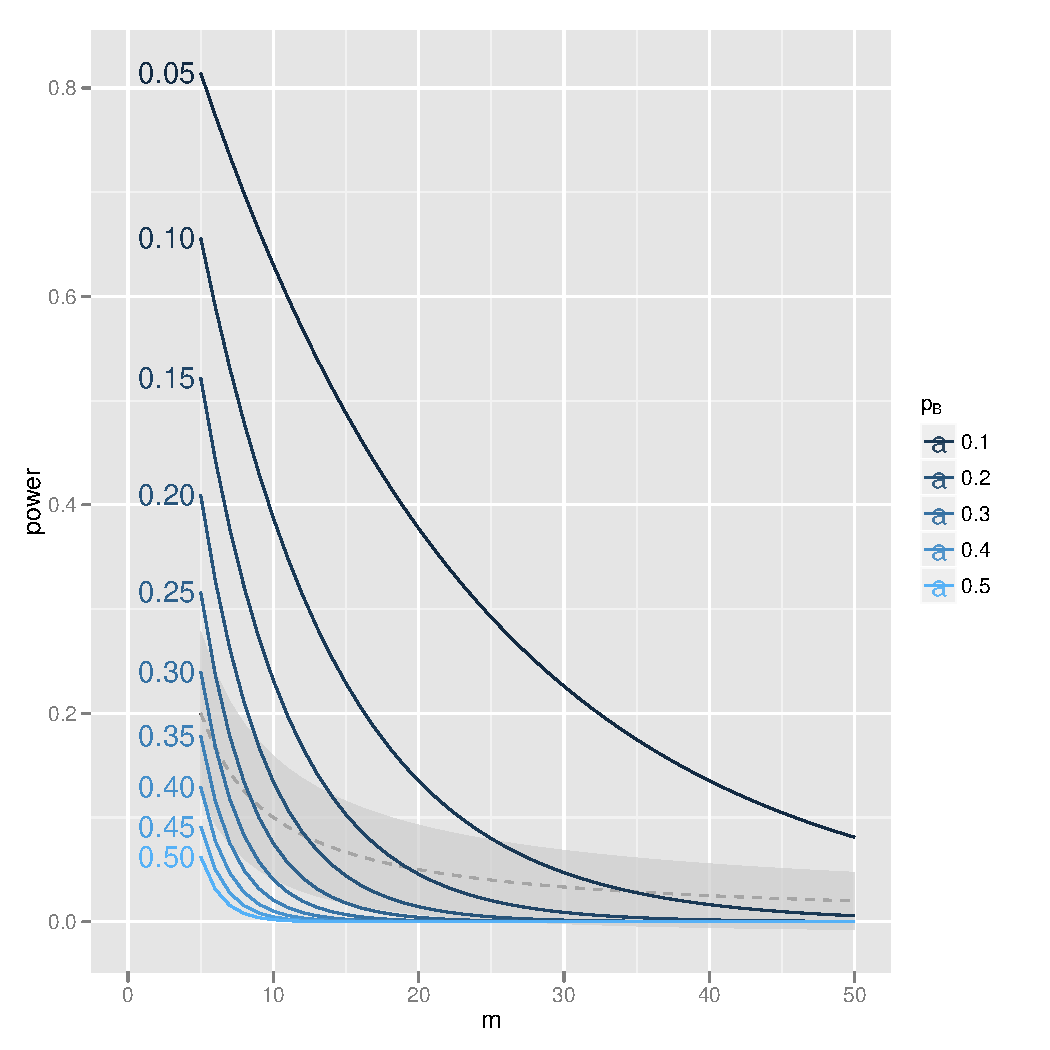
\includegraphics[width=2in]{images/powerplot.pdf} 
   \caption{Comparison of probabilities to pick the data plot for different size lineups $m$ and different values for data plot strength $p_B$. The grey line shows probability of picking the data plot under $H_0$.}
   \label{power}
\end{figure}



\end{document}  